\chapter{Applications and results}
\label{results}
The results of this project involve analysis of dynamical systems that describe chemical reactions, cell diffusion and complete  reaction-diffusion process as described in Chapter \ref{morphogenesis}. The latter is a set of linearised and non-linear models. The non-linear models are used to visualise cell structures and to study mutations. Results also show the rationale behind sound generation and some attempts to generate sound. Finally, the statistical information obtained from the scheduling algorithms demonstrate why scheduling using the concept of diffusion is promising. The results are obtained by the software applications that were developed for the project.
	\section{Chemical reactions}
Various chemical reactions were studied to identify how altering various parameters affects their behaviour. The main interest is to observe oscillatory behaviour, if any, and the amount of time needed for a reaction to be completed. Parameters are related to the concentration of each chemical substance, the reaction rate or coefficient which show the amount of each compound needed to produce another compound. 

    The experiments use the chemical reaction equations described by the Michaelis-Menten mechanism as presented in the case study of Stephen Childress \cite{childress_case_2005}. Four chemical substances are involved: one acting as a catalyst (enzyme E) interacting with a chemical substance X for composing the product P. There is a complex chemical compound C as a middle state which breaks into E+X or E+P according to the reaction rates $ k_{-1} $, and $ k_{+2} $ respectively. Note that the index in each rate k indicates the step (backwards, forward) needed to reach a certain state of the reaction.

The chemical reaction equation of the Michaelis-Menten mechanism is:
\begin{equation}
\label{excheq}
 E + X \underset{\underset{k_{-1}} \gets}{\overset{\overset{k_{+1}} \to}{}}  
		 C \overset{k_{+2}} \to E + P
\end{equation}

It is important to note that predictions are made before running an experiment. This helps in both testing and building an understanding of how, in this example, a complex reaction works.

\subsubsection{Prediction}

It is clear from the equation (\ref{excheq}) that the final products will be the enzyme E and the product P. The question arising is how can the maximum possible concentration of P be retrieved at the minimum amount of time? 

The complex compound C breaks into E and X at a rate $ k_{-1} $ into E and P at a rate $ k_{+2} $. When X runs out the reaction stops. Thus, the rate $ k_{+2} $ must be greater or equal to $ k_{-1} $ to accomplish the minimum time.

Table \ref{tableChemExp} shows the parameters of the try-outs for testing the Michaelis-Menten mechanism as described by the chemical equation (\ref{excheq}). 
\begin{table}
\begin{center}
\caption{Parameters used by solving the chemical equation (\ref{excheq}).}
\label{tableChemExp}
    \begin{tabular}{| c | c | c | c | c | c | c | c | c | c | c | c |}
        \hline
         & \multicolumn{4}{| c |}{Initial Concentrations} & \multicolumn{3}{| c |}{Reaction rates} \\ \hline
        Experiment Number & E & X & C & S & $ k_{+1} $ & $ k_{-1} $ & $ k_{+2} $ \\ \hline
        1 & 20 & 20 & 0 & 0 & 0.01 & 0.01 & 0.01 \\ \hline
        2 & 20 & 20 & 0 & 0 & 0.01 & 0.1 & 0.01 \\ \hline
        3 & 20 & 20 & 0 & 0 & 0.01 & 0.01 & 0.1 \\ \hline
        4 & 20 & 20 & 0 & 0 & 0.1 & 0.01 & 0.01 \\ \hline   
    \end{tabular}
\end{center}

\end{table}

\begin{figure}
\centering
\includegraphics[width=15cm, height=10cm]{exp2ch.png}
\caption{Graph showing the behaviour of the chemical reaction when there is a balance in all rates (experiment 1,Table \ref{tableChemExp}).}
\label{exp2ch1}
\end{figure}

\begin{figure}
\centering
\includegraphics[width=15cm, height=10cm]{exp2ch2.png}
\caption{Graph showing how a higher rate of C breaking into X affects Michaelis-Menten mechanism (experiment 2, Table \ref{tableChemExp}).}
\label{exp2ch2}
\end{figure}

\begin{figure}
\centering
\includegraphics[width=15cm, height=10cm]{exp2ch3.png}
\caption{Graph showing how a higher rate of C producing product P affects the Michaelis-Menten mechanism (experiment 3, Table \ref{tableChemExp}).}
\label{exp2ch3}
\end{figure}

\begin{figure}
\centering
\includegraphics[width=15cm, height=10cm]{exp2ch4.png}
\caption{Graph showing how a higher rate of producing C affects the Michaelis-Menten mechanism (experiment 4, Table \ref{tableChemExp}).}
\label{exp2ch4}
\end{figure}

The rationale behind the parameter values is based on discovering how each parameter affects the reaction. Starting with equal reaction rates and then changing only one parameter for each test, the altered behaviour can lead to conclusions which may verify the predictions. If the prediction is proven wrong, then either there is a bug in the code which integrates the differential equations or the logic behind the prediction was false or the mathematical model that described the chemical reaction was wrong.

The results show that, as predicted, that the higher the rate in which C breaks to E and P the less time is needed for chemical X to run out and cause the reaction to end. At the same time the production of E and X must be lower. So, generally the significance at the difference between $ k_{+2} $ and $ k_{-1} $ affects the overall production rate of P. The reaction rate of the production of the complex compound C also affects the time the reaction needs to complete. It can be high enough to satisfy the production rates of both ends. However, if it exceeds a certain threshold it has no effect, as the production rates of X and P are not sufficient to cover the concentration of C. 

The experiments from chemical reactions show that:
\begin{itemize}
\item The chemical reactions can be easily modelled with differential equations.
\item Compounds that break into different chemical substances present more complex behaviours and are closest to produce oscillations rather than equations of the form showed in the first example.
\item Different reaction rates affect the time for the completion of a chemical reaction but values exceeding a threshold may exist that have no effect.
\end{itemize}
   

\section{Diffusion}
Diffusion depends on the interconnections between cells. Two types of interconnection were studied: cells connected in a ring-shaped structure and a torus-shaped connection. The difference between the two is the number of cells each cell is attached to. In a ring, two cells are attached to every other cell. In a torus, four cells are attached to every other cell.

Diffusion was implemented according to the conduction of heat as described in Section \ref{diffusion}.
Experiments were done to identify the role of the parameters of the cells, the diffusion coefficients and the shape of the system. Table \ref{diffexp2} shows the parameters under study and figures \ref{d1}-\ref{d4} show the graph representations of the behaviour of such system.

The expected result after the diffusion process ends is that every cell has the same concentration of a particular morphogen as shown in figures \ref{d1}-\ref{d4}. The diffusion coefficient and the size of the cell affect the fluid flow and therefore smaller cells need more time to diffuse. The properties of a ring structure against a torus structure are also studied.

\begin{table}
\begin{center}
\caption{Parameters used to run tests on diffusion.}
\label{diffexp2}    
\begin{tabular}{| c | c | c | c | c | c |}
        \hline        
        No. & Cell side size & Number of Cells & Shape & Diffusion Coeff. & Initialisation method \\ \hline
        1 & 0.5 & 3 & Ring & 0.1 & Random \\ \hline
        2 & 0.1 & 3 & Ring & 0.1 & Random \\ \hline
        3 & 0.5 & 9 & Ring & 0.1 & Random \\ \hline
        4 & 0.5 & 4 & Torus & 0.1 & Random \\ \hline
    \end{tabular}
\end{center}
\end{table}

\begin{figure}
\centering
\includegraphics[width=15cm, height=10cm]{diffusion1.png}
\caption{Graph showing chemical concentrations during the diffusion process (experiment 1, Table \ref{diffexp2}).}
\label{d1}
\end{figure}


\begin{figure}
\centering
\includegraphics[width=15cm, height=10cm]{diffusion2.png}
\caption{Graph showing how the size of the cells affects the diffusion process (experiment 2, Table \ref{diffexp2}).}
\label{d2}
\end{figure}

\begin{figure}
\centering
\includegraphics[width=15cm, height=10cm]{diffusion3.png}
\caption{Graph showing how the number of the cells affects the diffusion process (experiment 3, Table \ref{diffexp2}).}
\label{d3}
\end{figure}

\begin{figure}
\centering
\includegraphics[width=15cm, height=10cm]{diffusion4.png}
\caption{Graph showing the diffusion process in a torus structure (experiment 4, Table \ref{diffexp2}).}
\label{d4}
\end{figure}

Conclusions obtained from the results of tests 2, 3 and 4 compared to 1 (Table \ref{diffexp2}):
\begin{itemize}
\item Experiment 2 shows that with smaller cells, diffusion needs more time to be completed.
\item Experiment 3 shows that more cells need more time to complete the diffusion process.
\item Experiment 4 shows that a torus structure diffuses faster that a ring one.     
\end{itemize}
		
\section{Reaction-diffusion}
    Reaction-diffusion models can be considered as complete models of morphogenesis. They result from merging reaction and diffusion models. Depending on the type of the function, linear or non-linear, that describes a chemical reaction, the models are categorised into linear or non-linear.
    
The linearised model that is tested in Section \ref{resLinear} produces negative solutions as well. Negative solutions are not accepted when working with chemical substances, since a negative concentration does not have a physical meaning. There is an option for forcing the ODE solver to always produce non-negative solutions. However, this results in unstable behaviour. Nevertheless, as explained in Section \ref{linsys} the goal is to approximate the behaviour of a system near the equilibrium points. In other words, the study is about the qualitative behaviour of the system rather than the quantitative one.

Modelling with non-linear systems gives an approximation closer to reality since chemical substances can't be negative. Results for non-linear systems include image snapshots of the cell structure at particular time points.

    
\subsection{Implementing and testing with linearised models}
\label{resLinear}
The linear system that was studied is proposed by Alan Turing \cite{turing_chemical_1990} and analysed in the case study of Stephen Childress \cite{childress_case_2005}. The main interest lies on the stability conditions. The equation is of the form:
$$ \dot{x} = Ax $$
Where A is the Jacobian matrix evaluated at the equilibrium point as described in  \ref{linsys} and has size $ N\times N $.
The case studies a system with 2 morphogens. 
$$ N=2,$$
$$ A \in \mathbb{R}^{2\times 2} $$

The stability conditions are computed by finding the roots of the characteristic equation obtained from equation (\ref{char}) and analysed in \cite[p.~5]{childress_case_2005} computing the conditions shown in equation (\ref{conditionsA}).
\begin{equation}
\label{jacobian}
A= 
\begin{pmatrix}
        a_{11} & a_{12} \\
        a_{21} & a_{22} \\
\end{pmatrix}
\end{equation}

\begin{equation}
\label{char}
det(A-\lambda I) = 0 
\end{equation}

$$a_{11} + a_{22} < 0,$$
\begin{equation}
\label{conditionsA}  
 a_{11}a_{22} - a_{12}a_{21} > 0
\end{equation}


In other words, the linearised matrix can have several random forms, but always satisfy the given conditions in \ref{conditionsA}. The program in Appendix Section \ref{initialisea} is responsible for the generation of such random matrices. Table \ref{linexp} shows the different values of the matrix. The Figures \ref{l1}-\ref{l4} show the behaviour of the system. Note that the Jacobian matrix is used to approximate the behavior of the reaction process. Merging the corresponding matrix with the diffusion in a ring of cells from equation (\ref{diffeq}), the system becomes as shown by equation (\ref{lrdm}).

\begin{equation}
\label{lrdm}
\dot{x}_i = Ax_i + \begin{pmatrix}
\delta^2d_1 & 0 \\
0 & \delta^2d_2 \\
\end{pmatrix}(x_{leftof(i)} - 2x_i + x_{rightof(i)})
\end{equation}

\begin{table}
\begin{center}
\caption{Experiments using the Jacobian matrix and diffusion for modelling the process of reaction-diffusion in a ring of cells.}
\label{linexp}
\begin{tabular}{| c | c | c | c | c | c |}
\hline
No. & A & No. of cells & Diffusion included & Initial state & Satisfies conditions\\ \hline
1 & $ \begin{pmatrix}
        0.6171 & 0.8244 \\
        -1.6432 & -0.8824 \\
\end{pmatrix} $ & 3 & Yes & Random & Yes\\ \hline
2 & $\begin{pmatrix}
        0.6834 & 0.4423 \\
        -2.1634 & -1.3875 \\
\end{pmatrix} $ & 3 & Yes & Random & Yes\\ \hline
3 & $\begin{pmatrix}
        -1.6364 & 0.8824 \\
        -0.5 & -0.312 \\
\end{pmatrix} $ & 3 & Yes & Random & No \\ \hline
4 & $ \begin{pmatrix}
        0.6171 & 0.8244 \\
       -1.6432 & -0.8824 \\
\end{pmatrix} $ & 3 & No & Random & Yes \\ \hline
\end{tabular}
\end{center}
\end{table}

\begin{figure}
\centering
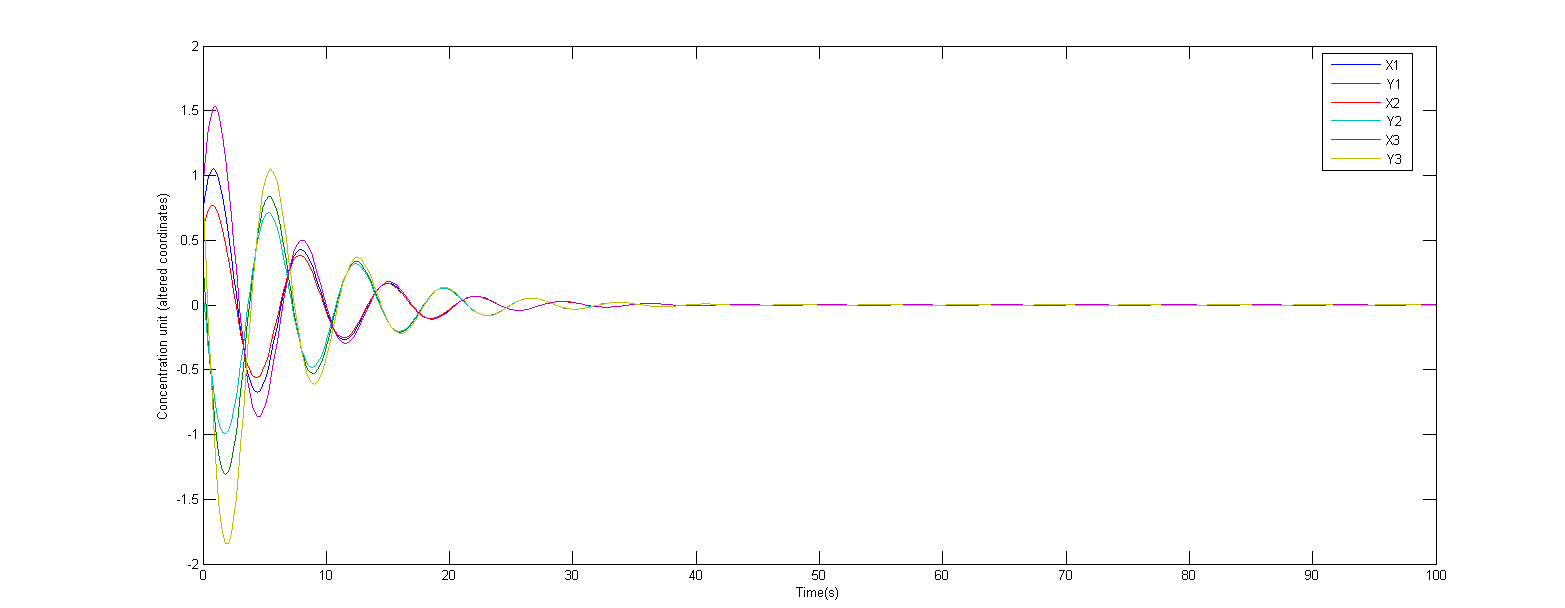
\includegraphics[width=15cm, height=10cm]{l1.png}
\caption{Graph showing the behaviour of a linear reaction-diffusion system (experiment 1, Table \ref{linexp}).}
\label{l1}
\end{figure}

\begin{figure}
\centering
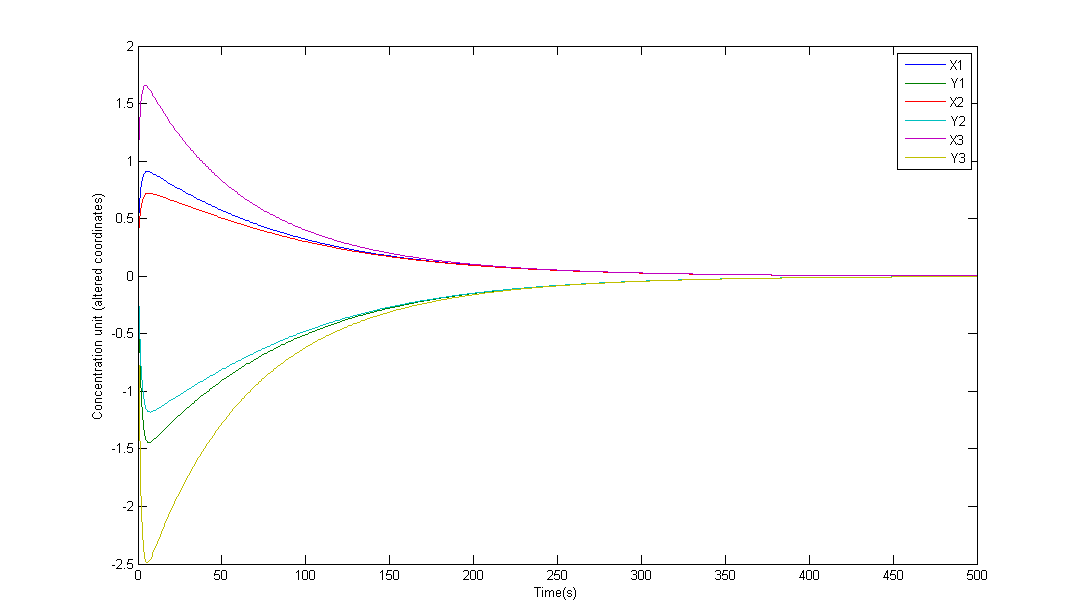
\includegraphics[width=15cm, height=10cm]{l2.png}
\caption{Graph showing the behaviour of a linear reaction-diffusion system with different values of the Jacobian matrix (experiment 2, Table \ref{linexp}).}
\label{l2}
\end{figure}

\begin{figure}
\centering
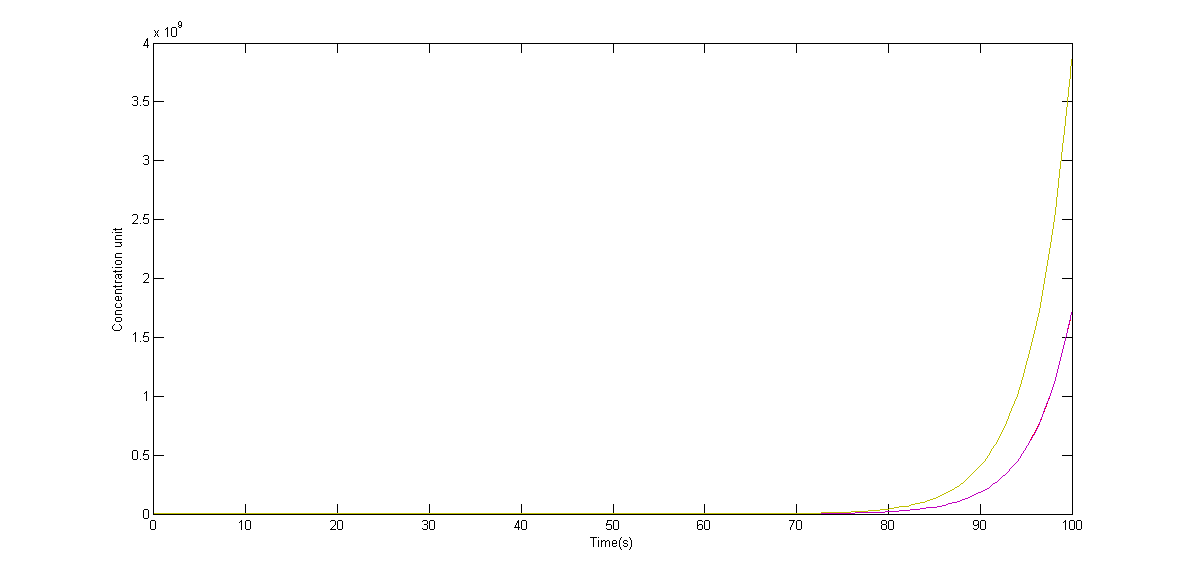
\includegraphics[width=15cm, height=10cm]{l3.png}
\caption{Graph showing that a linearised reaction-diffusion system is unstable if stability conditions are not satisfied (experiment 3 from Table \ref{linexp}).}
\label{l3}
\end{figure}

\begin{figure}
\centering
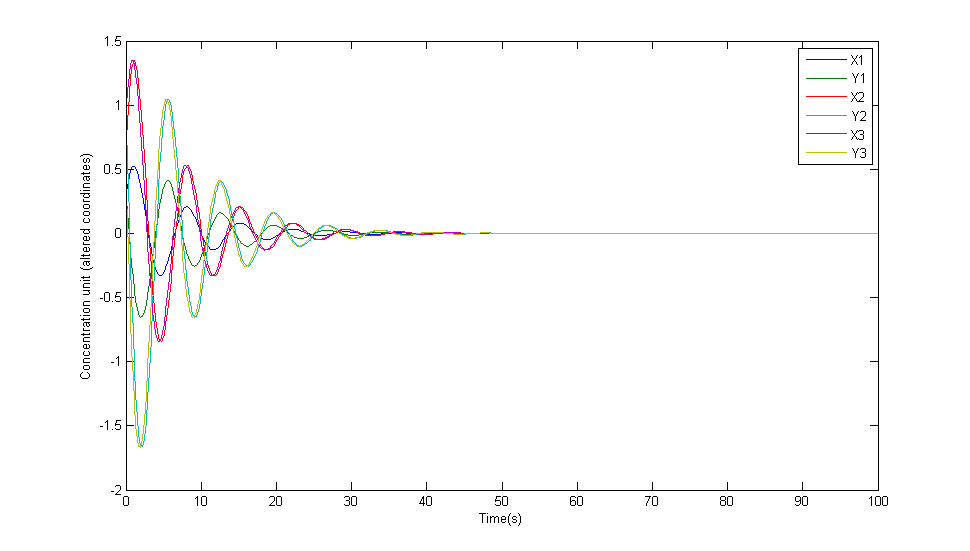
\includegraphics[width=15cm, height=10cm]{l4.png}
\caption{Graph showing the same linear system as in experiment 1 but without diffusion (experiment 4, Table \ref{linexp}).}
\label{l4}
\end{figure}

The experiments show that:
\begin{itemize}
\item The absence of diffusion as opposed in experiment 4 of table \ref{linexp} does not affect the oscillatory behaviour.
\item Not satisfying the stability conditions leads to an unstable system with infinity values, as shown in test 3 of table \ref{linexp}.
\end{itemize}

Results do not prove or show regarding the way that diffusion affects the system. Trying to perform the same tests by changing the diffusion coefficients only is shown in Table \ref{diffLexp} and figures \ref{ld1}, \ref{ld2} opposed to \ref{l1} and \ref{l2} respectively. 

\begin{table}
\caption{Experiments on how a linear system is affected from diffusion.}
\label{diffLexp} 
\begin{center}
\begin{tabular}{| c | c | c | c | c |}
\hline
No. & A & No. of cells & {Diffusion coefficients (M)} & Initial state\\ \hline
1 & $ \begin{pmatrix}
        0.6171 & 0.8244 \\
        -1.6432 & -0.8824 \\
\end{pmatrix} $ & 3 & 
$ \begin{pmatrix}
        0.025 & 0 \\
        0 & 0.05 \\
\end{pmatrix} $
 & Random \\ \hline


2 & $ \begin{pmatrix}
        0.6171 & 0.8244 \\
        -1.6432 & -0.8824 \\
\end{pmatrix} $ & 3 & 
$ \begin{pmatrix}
        2.5 & 0 \\
        0 & 5 \\
\end{pmatrix} $
 & Random \\ \hline


3 & $\begin{pmatrix}
        0.6834 & 0.4423 \\
        -2.1634 & -1.3875 \\
\end{pmatrix} $ & 3 & 
$ \begin{pmatrix}
        0.025 & 0 \\
        0 & 0.05 \\
\end{pmatrix} $ 
& Random \\ \hline


4 & $\begin{pmatrix}
        0.6834 & 0.4423 \\
        -2.1634 & -1.3875 \\
\end{pmatrix} $ & 3 & 
$ \begin{pmatrix}
        40 & 0 \\
        0 & 80 \\
\end{pmatrix} $ 
& Random \\ \hline
\end{tabular}
\end{center}
\end{table}


\begin{figure}
\centering
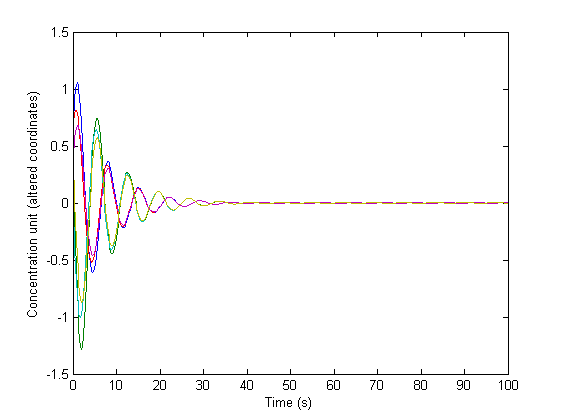
\includegraphics[width=15cm, height=10cm]{ld1.png}
\caption{Graph showing how the behaviour of the linear system differantiates with large diffusion coefficients (experiment 2, Table \ref{diffLexp} opposed to experiment 1, Figure \ref{l1}).}
\label{ld1}
\end{figure}

\begin{figure}
\centering
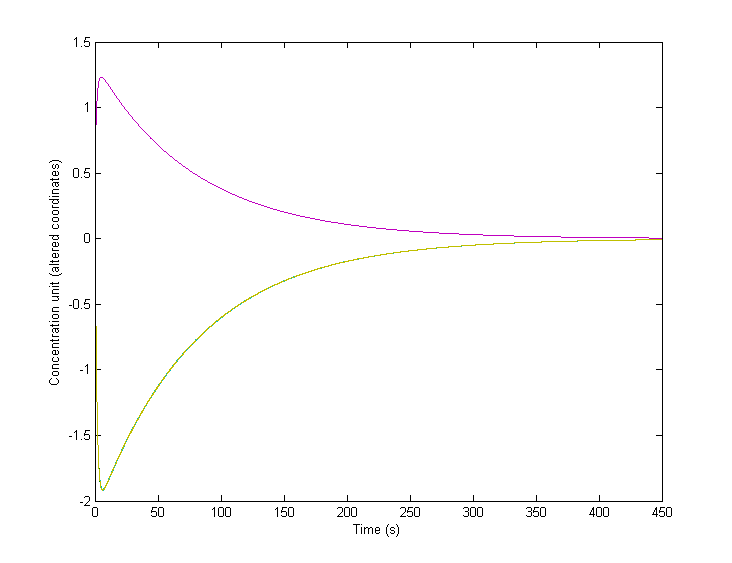
\includegraphics[width=15cm, height=10cm]{ld2.png}
\caption{Graph showing how the behaviour of the linear system differantiates with very large diffusion coefficients (experiment 4, Table \ref{diffLexp} opposed to experiment 3, figure \ref{l2}).}
\label{ld2}
\end{figure}

Notice now that only two colours are visible in the graph \ref{l2}. That means that morphogen concentrations in cells are equal and thus, with high diffusion coefficients (40 and 80) all cells rapidly become identical. This means that large diffusion coefficients must be avoided in order to differentiate cells.

The general conclusion is that diffusion is very important in morphogenesis and has a high impact on the behaviour of the system. Despite the fact that graphs show identical behaviour, it should not be neglected that the purpose of the project is to generate software applications that present how cells create structures. Cells must have properties that differentiate one-another. By setting a large diffusion coefficient value, cells may become quickly identical and the internal chemical reactions will not lead into different results. The choice of diffusion coefficients is therefore critical.


\subsection{Non-linear models}
\label{resnonlinear}
The non-linear models discussed in Chapter \ref{morphogenesis} were used to the final software solutions. The main purpose was to show how cells are organising and form structures out of a random chaotic state. The results are shown in images that represent the structure of the system. Those images are snapshots of the system at time zero, middle and final point snapshots are arranged in a timeline. 

Table \ref{rdtable} shows the parameters and the models that were used. Notice that diffusion coefficients and the number of cells affect the structure of the system. 

\begin{table}
\begin{center}
\caption{Experiments of non-linear models with various parameters.}
\label{rdtable}
\begin{tabular}{| c | c | c | c | c |}
\hline
No. & Model & Parameters & Diffusion Coefficients & Number of Cells \\ \hline
1 & L-Systems & None & $ D_u=1.6, D_v=6 $ & 6400 \\ \hline
2 & L-Systems & None & $ D_u=1.6 $,$ D_v=6 $ & 22500 \\ \hline
3 & L-Systems & None & $ D_u=3.5 $, $ D_v=16 $ & 6400 \\ \hline
4 & L-Systems & None & $ D_u=2 $, $ D_v=5 $ & 6400 \\ \hline
5 & Gray Scott & $ F=40 $,$ k=60 $ & $ D_u=1 $, $ D_v=16 $ & 22500 \\ \hline
6 & Gray Scott & $ F=30 $,$ k=40 $ & $ D_u=1 $, $ D_v=16 $ & 22500 \\ \hline
\end{tabular}
\end{center}
\end{table}

\begin{figure}
\begin{center}
\includegraphics[width=4cm, height=4cm]{rd11.png}
\includegraphics[width=4cm, height=4cm]{rd12.png}
\includegraphics[width=4cm, height=4cm]{rd13.png}
\end{center}
\caption{Initial, middle and final snapshots of the structure of the L-systems of experiment No. 1, Table \ref{rdtable}.}
\label{rd1}
\end{figure}

\begin{figure}
\begin{center}
\includegraphics[width=4cm, height=4cm]{rd21.png}
\includegraphics[width=4cm, height=4cm]{rd22.png}
\includegraphics[width=4cm, height=4cm]{rd23.png}
\end{center}
\caption{Initial, middle and final snapshots of the structure of the L-systems with more cells as shown in experiment 2, Table \ref{rdtable}.}
\label{rd2}
\end{figure}

\begin{figure}
\begin{center}
\includegraphics[width=4cm, height=4cm]{rd31.png}
\includegraphics[width=4cm, height=4cm]{rd32.png}
\includegraphics[width=4cm, height=4cm]{rd33.png}
\end{center}
\caption{Initial, middle and final snapshots of the structure of the L-systems with different diffusion coefficients (experiment 3, Table \ref{rdtable}).}
\label{rd3}
\end{figure}

\begin{figure}
\begin{center}
\includegraphics[width=4cm, height=4cm]{rd41.png}
\includegraphics[width=4cm, height=4cm]{rd42.png}
\includegraphics[width=4cm, height=4cm]{rd43.png}
\end{center}
\caption{Initial, middle and final snapshots of the structure of the L-systems with different diffusion coefficients (experiment 4, Table \ref{rdtable}).}
\label{rd4}
\end{figure}

\begin{figure}
\begin{center}
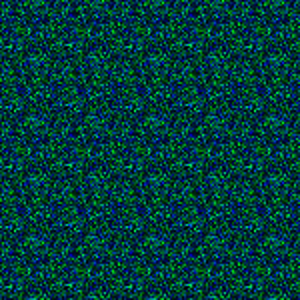
\includegraphics[width=4cm, height=4cm]{gs11.png}
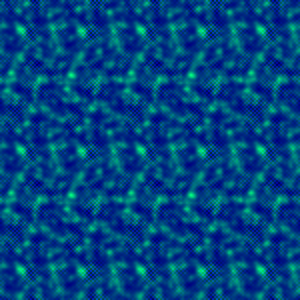
\includegraphics[width=4cm, height=4cm]{gs12.png}
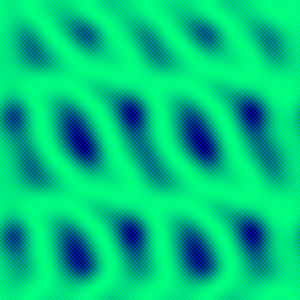
\includegraphics[width=4cm, height=4cm]{gs13.png}
\end{center}
\caption{Initial, middle and final snapshots of the structure of the Gray-Scott model with parameters shown in experiment No.5, Table \ref{rdtable}.}
\label{gs1}
\end{figure}

\begin{figure}
\begin{center}

\includegraphics[width=4cm, height=4cm]{gs21.png}
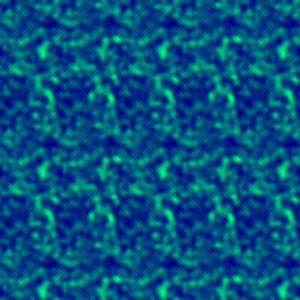
\includegraphics[width=4cm, height=4cm]{gs22.png}
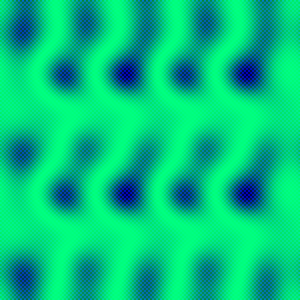
\includegraphics[width=4cm, height=4cm]{gs23.png}
\end{center}
\caption{Initial, middle and final snapshots of the structure of the Gray-Scott model with different reaction rates (experiment No.5, Table \ref{rdtable}).}
\label{gs2}
\end{figure}

As shown in Figures \ref{rd1}-\ref{gs2}, a variety of different structures is obtained. The cells start with a randomly initialised state, but they form shapes and patterns progressively in time.



\subsection{Introducing mutation}

A physical system in the real world is never isolated. External factors or random events might affect the cells by changing their state. This phenomenon is called mutation and one of the reasons, for example, for producing cancerous masses in advanced biological organisms or causing changes of characteristics (for instance, change in the eye colour). In some organisms, controlled mutations may have desirable effects. In agriculture, grafting takes place in plants to make them produce better fruit \cite{nelson_principles_2007}. Mutation occurs under different circumstances, but the concept remains the same; the behaviour of a system is changed by altering some of its properties.

A study on altering the system randomly after its development is proposed. The process is that the system is left to evolve for a specific amount of time. Then, random perturbations change some cells by altering their morphogen concentrations and the system is integrated again. The purpose is to find at what mutation probabilities the structure of the system is changed dramatically beyond recovery.

This can be done by observing the structures prior to and following mutation. Due to the colour mapping, a single cell mutation may lead to the false conclusion that the structure changed rapidly but this is not the case. What one should observe is whether the change in some cells can be absorbed by the system and if the system recovers to its previous structure.

\begin{table}
\begin{center}
\caption{Showing the effect of mutation on different probabilities.}
\label{muttable}
\begin{tabular}{| c | c | c | c | c |}
\hline
No. & Diffusion Coefficients & Number of Cells & Mutation Probability & Number of mutated cells \\ \hline
1 & $ D_u=1.6, D_v=6 $ & 3600 & 0.001 & 2 \\ \hline
2 & $ D_u=1.6, D_v=6 $ & 3600 & 0.01 & 39 \\ \hline
\end{tabular}
\end{center}
\end{table}

\begin{figure}
\begin{center}
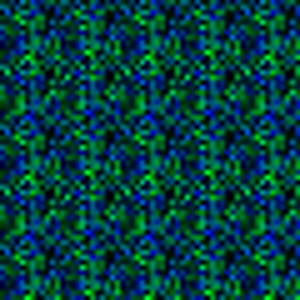
\includegraphics[width=4cm, height=4cm]{st1.png}
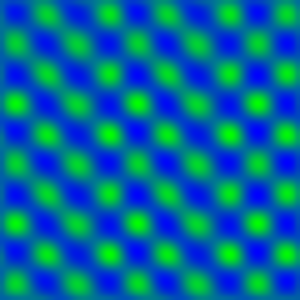
\includegraphics[width=4cm, height=4cm]{bm1.png}
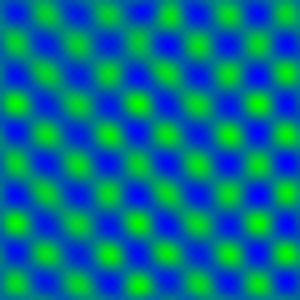
\includegraphics[width=4cm, height=4cm]{am1.png}
\end{center}
\caption{Initial state, final structure before mutation , and recovered structure after mutation with mutation probability 0.001 (experiment 1, Table \ref{muttable}).}
\label{mut1}
\end{figure}

\begin{figure}
\begin{center}
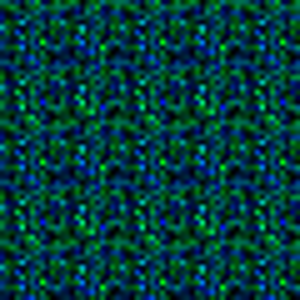
\includegraphics[width=4cm, height=4cm]{st2.png}
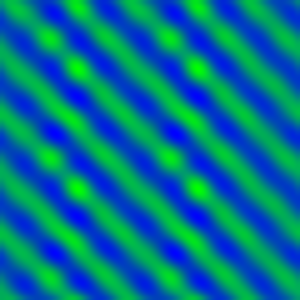
\includegraphics[width=4cm, height=4cm]{bm2.png}
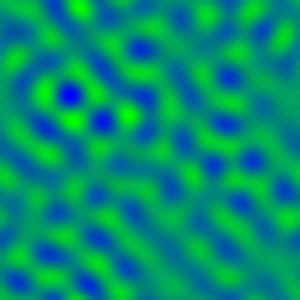
\includegraphics[width=4cm, height=4cm]{am2.png}
\end{center}
\caption{Initial state, final structure before and after mutation showing that with probability 0.01 the structure changes (experiment 2, Table \ref{muttable}).}
\label{mut2}
\end{figure}

The results show that a probability of cell mutation equal to 0.01 is sufficient to alter the final structure of a system. 

More ideas arise on how to experiment with mutation. One is to find the highest probability at which a system can recover. As shown, a probability of 0.01 caused the structure of the system to change while the probability of 0.001 did not affect the system. What may be the threshold that brings the system to its limit?

Another idea would be to simulate the method of grafting. In this method, a tissue is taken from a plant and is inserted into another one. That process may transform, for example, a part of a mandarin tree to become an orange tree. A similar approach can be used to visualise this concept. A way of accomplishing this could be to generate two structures. In practice, the structures are matrices, in theory they are systems of cells. Then, take from the two structures a portion (a column, a row, or a small square portion) of each and substitute them. How will each structure be after integration? This is an interesting experiment that expands the results of this section.


	\section{Producing sound}
\label{glsound}
Mathematical models of morphogenesis have oscillatory behaviour. Thus, they share a common behaviour with sound. The sinusoidal waves of a mathematical reaction-diffusion model can be converted into frequency spectra and then sound may be produced by driving the spectra values to the sound card.

A mathematical model that presents continuous waves is needed. The Gizburg-Landau was used as was analysed and implemented by Aly-Khan Kassam \cite{kassam_solving_2003}
Figure \ref{gl}
shows the pattern that this model generates.    

There are various ways for extracting frequency spectra values from the waves that the Gizburg-Landau model generates. The problem is the same with colour values: to find the right way for mapping the morphogen concentrations into frequency values. The method that was followed was to get the mean of the morphogen concentrations for each point in time. The result is shown in Figure \ref{soundspectra}.


\begin{figure}
\centering
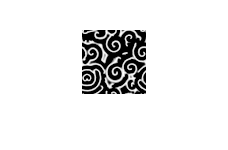
\includegraphics{gl.png}
\caption{Pattern produced by the Gizburg-Landau model.}
\label{gl}
\end{figure}

\begin{figure}
\centering
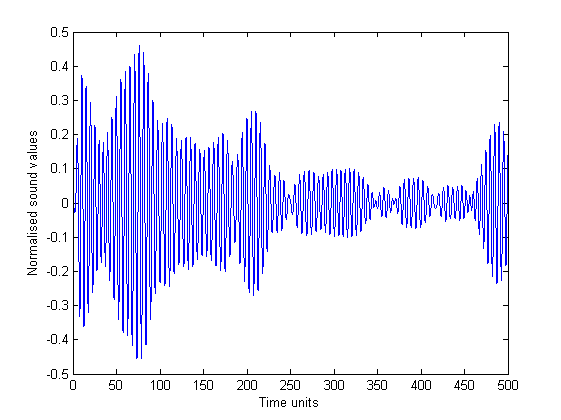
\includegraphics[scale=0.7]{sound_spectra.png}
\caption{Sound spectra by calculating the mean values of the morphogens.}
\label{soundspectra}
\end{figure}


	\section{Comparing schedulers}
\label{sca}
The scheduling solution described in Section \ref{schedulers}
involved four schedulers. The random scheduler, a priority scheduler, the Round Robin Scheduler and the project-related diffusion-scheduler. The results show a similar performance of the Round Robin and the Diffusion scheduler. As shown in the bar graph Figures \ref{schh}, \ref{schk}, \ref{fiveschk}, \ref{fifteenschk}
the diffusion-inspired scheduler can execute processes faster than the other schedulers.

However, the main problem is the complexity of the implementation of the Euler's method inside the scheduler which demotivates the import of the diffusion scheduler to a real operating system. Further study can be made on how it can be imported to a distributed system by handling concurrency.

Table \ref{schtable} shows a short amount of testing and statistical analysis which proves why further study on diffusion-inspired scheduling is needed.  

\begin{table}
\caption{Experiment parameters for testing the diffusion-inspired scheduler against other schedulers.}
\label{schtable}
\begin{center}
\begin{tabular}{| c | c | c |}
\hline
No. & Diffusion Coefficient &  Number of Processes \\ \hline
1 & 1 & 100 \\ \hline
2 & 1 & 1000 \\ \hline
3 & 5 & 1000 \\ \hline
4 & 15 & 1000 \\ \hline
\end{tabular}
\end{center}
\end{table}

\begin{figure}
\centering
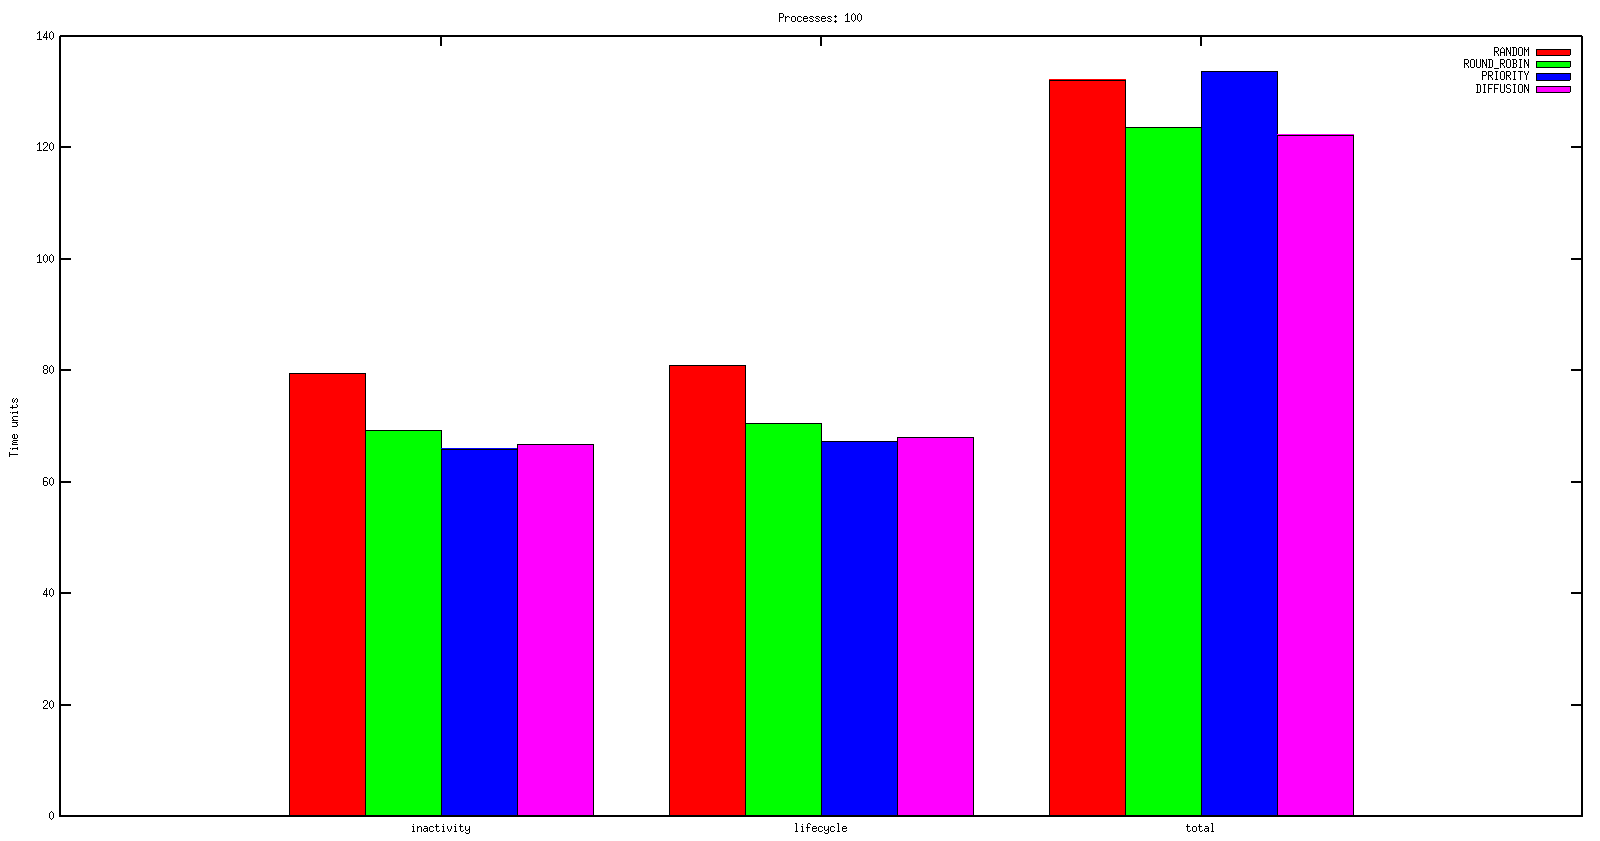
\includegraphics[scale=0.3]{sch100.png}
\caption{Comparison of the scheduler implementations with 100 processes in the queue (experiment No. 1 of Table \ref{schtable}).}
\label{schh}
\end{figure}

\begin{figure}
\centering
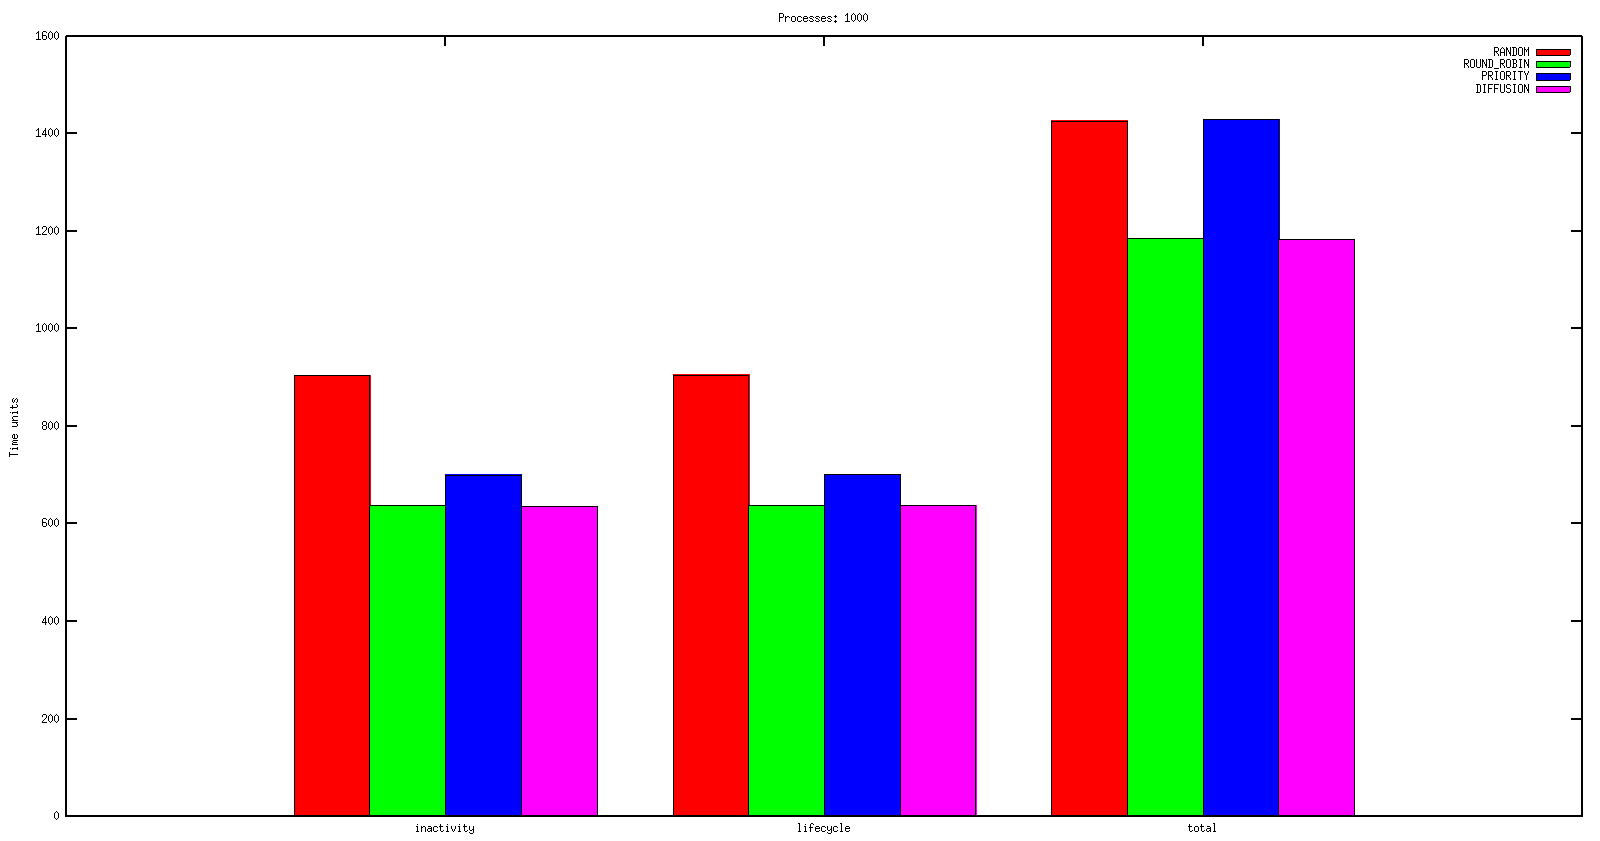
\includegraphics[scale=0.3]{sch1000.png}
\caption{Comparison of the scheduler implementations with 1000 processes in the queue (experiment No. 2 of Table \ref{schtable}).}
\label{schk}
\end{figure}

\begin{figure}
\centering
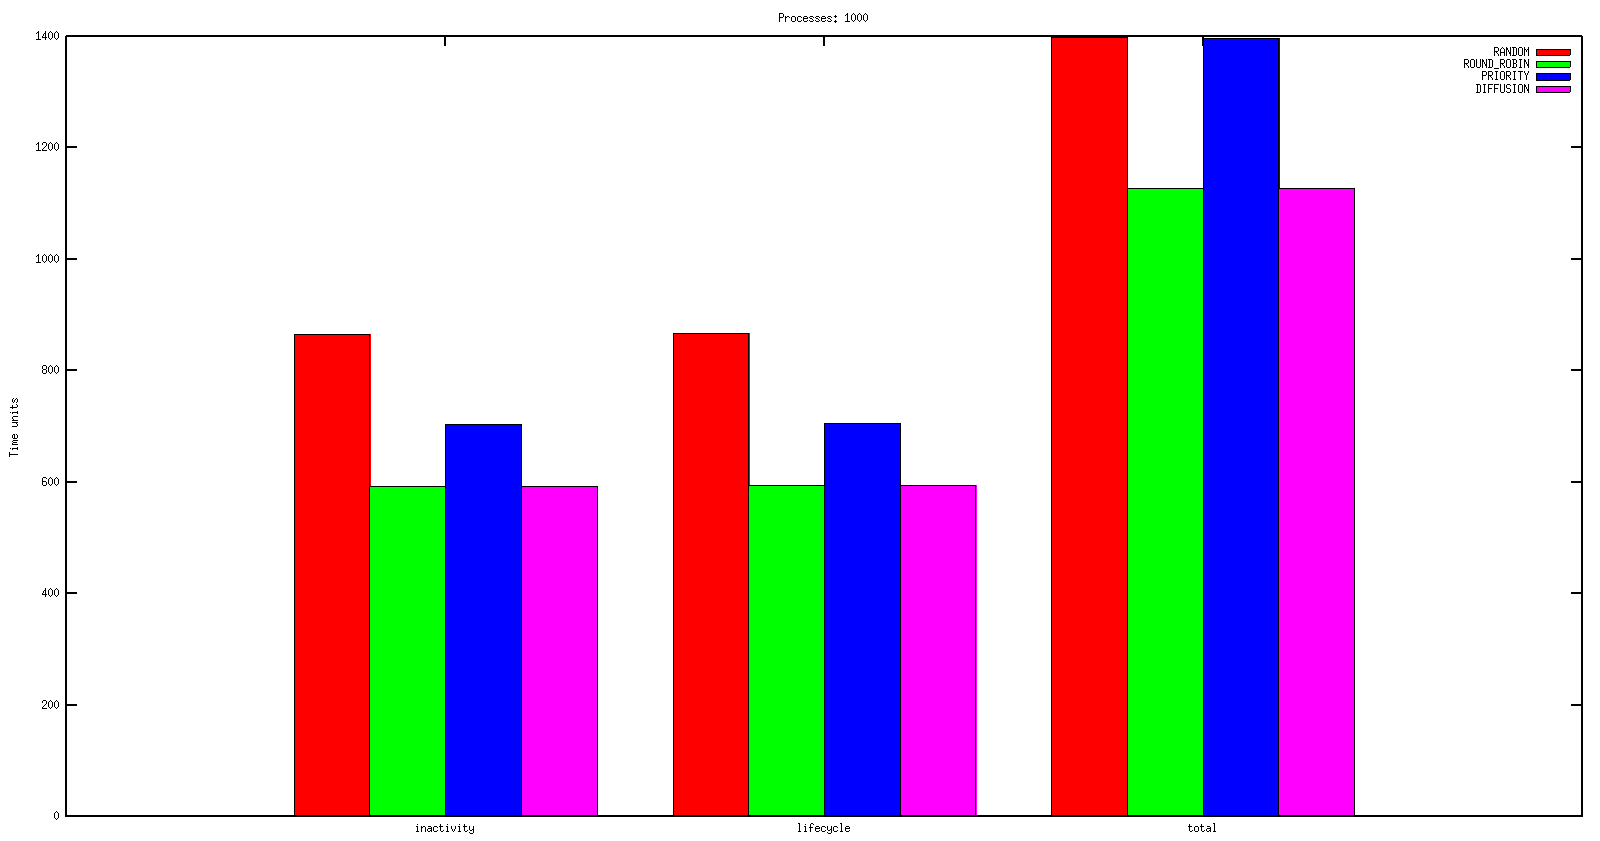
\includegraphics[scale=0.3]{5sch1000.png}
\caption{Comparison of the scheduler implementations with 1000 processes in the queue and a different diffusion coefficient (5) for the diffusion-inspired scheduler (experiment No. 3 of Table \ref{schtable}).}
\label{fiveschk}
\end{figure}

\begin{figure}
\centering
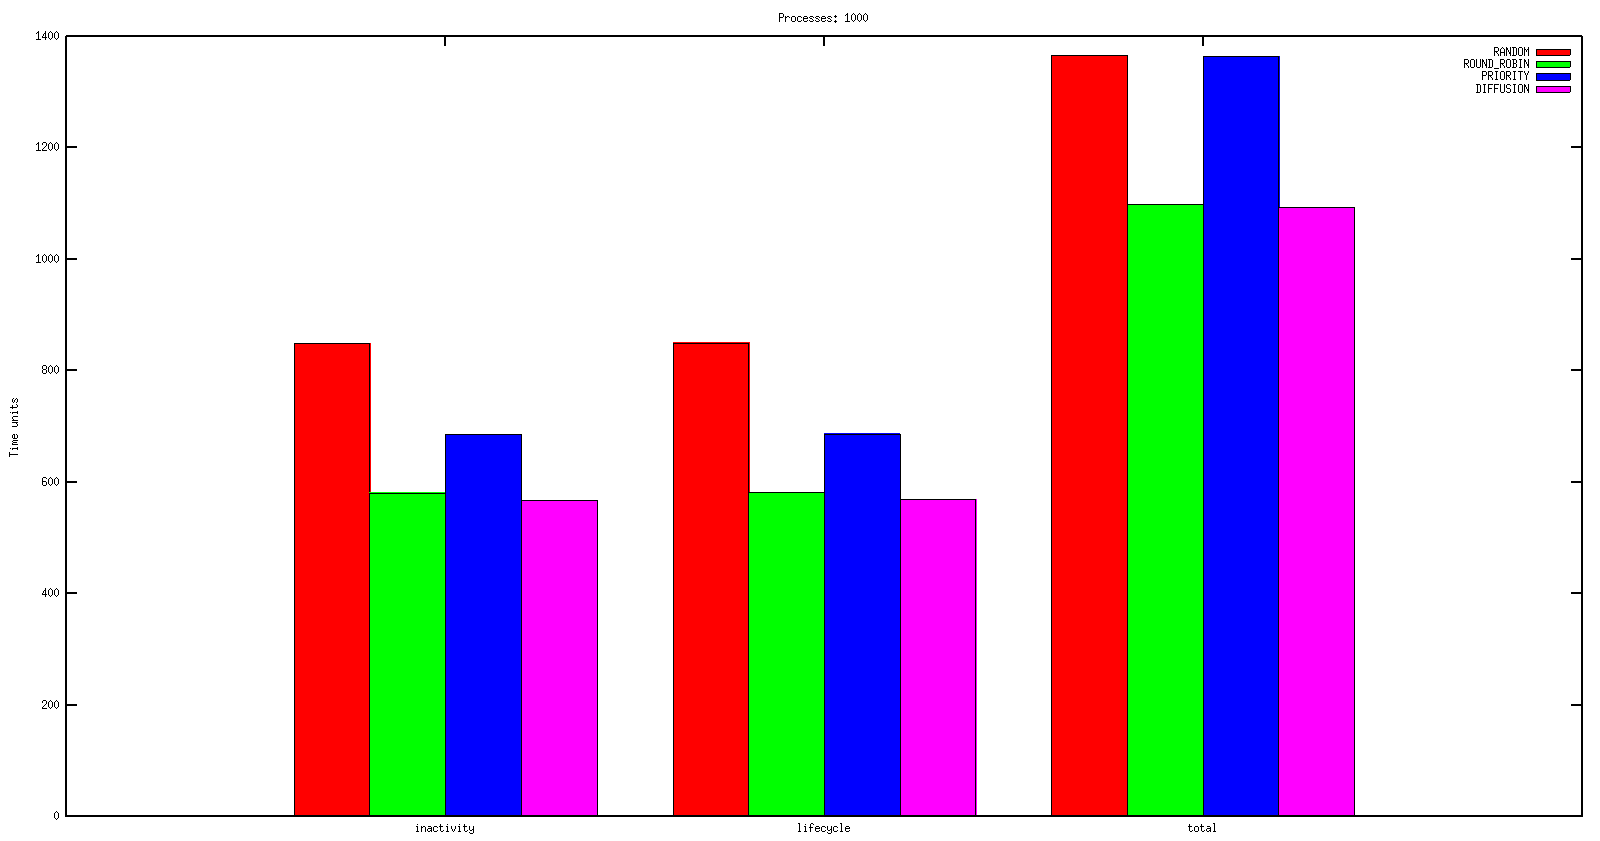
\includegraphics[scale=0.3]{15sch1000.png}
\caption{Comparison of the scheduler implementations with 1000 processes in the queue and the diffusion coefficient of the diffusion-inspired scheduler being 15 (experiment No. 4 of Table \ref{schtable}).}
\label{fifteenschk}
\end{figure}
		
